%!TEX root = ../main.tex
%
\section[Delta robot]{Delta robot}
\begin{frame}
\frametitle{Delta robot}
The Delta robot is a 3-DOF parallel kinematic machine developed by Reymond Clavel~\footfullcite{Clavel1991} in 1991. It mainly consists of three actuated kinematic chains linked at a common moving platform. Each chain is a serial connection of a revolute actuator, a rear-arm and a forearm (composed of two parallel rods forming a parallelogram). The rear-arms and the forearms are linked through ball-and-socket passive joints. The parallelogram structure of the forearms ensures that the moving platform stays always parallel to the fixed base.
Figure~\ref{fig:Delta_schematic} shows a schematic view of the Delta robot with its main elements highlighted.
\end{frame}
%
\begin{frame}
\frametitle{Delta robot - Schematic view}
\begin{columns}
    \begin{column}{0.5\textwidth}
		\vspace*{.6 cm}
    	\begin{figure}
    		\frame{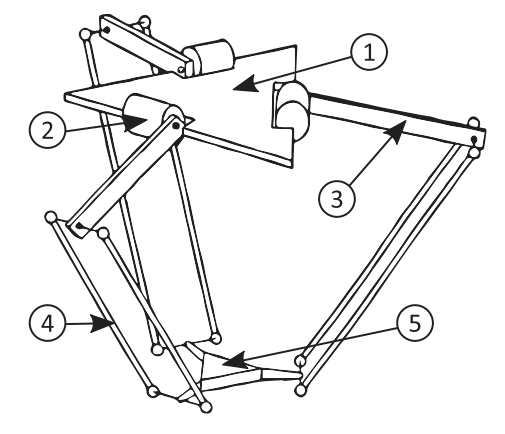
\includegraphics[width=.8\linewidth]{img/Delta.png}}
    		\caption{Schematic view of Delta robot}
    		\label{fig:Delta_schematic}
    	\end{figure}
    \end{column}
    \begin{column}{0.5\textwidth}
        \begin{enumerate}
        	\item Fixed base-plate
        	\item Actuator
        	\item Rear-arm
        	\item Forearm
        	\item Moving platform
        \end{enumerate}
    \end{column}
\end{columns}
We consider a model with a ternary symmetric configuration with three kinematic chains disposed with a period of $120\degree$.
\end{frame}
%
\begin{frame}
\frametitle{Delta robot - Parameters}
	\begin{figure}
		\frame{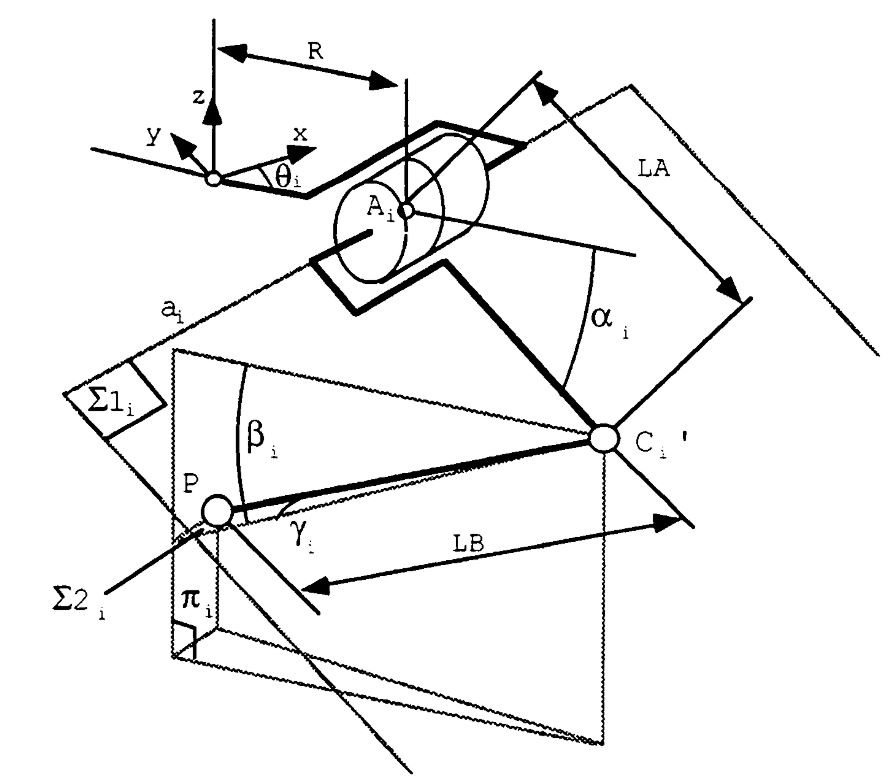
\includegraphics[width=.6\linewidth]{img/DeltaRobotClavelpg26.JPG}}
		\caption{Delta robot length parameters and characteristic angles}
		\label{fig:Delta_param}
	\end{figure}
\end{frame}
%
\begin{frame}
\frametitle{Delta robot - Parameters}
\begin{table}
\begin{center}
\begin{tabu} to \textwidth { | X[c] | X[c] | X[c] | }
	\hline
	\textbf{Parameter} & \textbf{Description} & \textbf{Value} \\
	\hline
	$l_A$ & Rear-arm length & $0.2 m$ \\
	$m_A$ & Rear-arm mass & $0.1 Kg$ \\
	$R$ & Base platform dimension & $0.126 m$ \\
	$l_B$ & Forearm length & $0.4 m$ \\
	$m_B$ & Forearm mass & $0.045 Kg$ \\
	$m_c$ & Elbow mass & $0.018 Kg$ \\
	$m_n$ & Moving platform mass & $0.1 Kg$ \\
	$I_{bi}$ & Rear-arm inertia & $Kg\times m^2$ \\
	\hline
\end{tabu}
\caption{Delta robot geometric and dynamic parameters}
\label{tab:Delta_param}
\end{center}
\end{table}
\end{frame}
%
\begin{frame}
\frametitle{Delta robot - Parameters}
Analytical studies on the working volume of the Delta robot~\footfullcite{Rey} showed that:
\begin{itemize}
 	\item A ratio $r = R/l_A < 0.63$ gives the most regular shape for the surface of the lower part of the working volume.
 	\item If $r > 0.0484$ and $b = l_A/l_B > 1.75$ there is no singularity occurrence within the robot working volume.
\end{itemize}
Thus the parameters shown in table~\ref{tab:Delta_param} have been chosen for the Delta model used in this project.
\end{frame}
%
\begin{frame}
\frametitle{Delta robot - Reference system and state variables}
The position of the End-effector
\[
(x,y,z)^T
\]
is described in a reference frame fixed to the base plate, as shown in figure~\ref{fig:Delta_param}.\\
\vspace{.5cm}
The angles $\alpha_i$ of the actuated joints have been selected as state-variables to describe the robot dynamic:
\[
q = (\alpha_1, \alpha_2, \alpha_3)^T
\]

\end{frame}
%
\subsection{Direct kinematic}
%
\begin{frame}
\frametitle{Delta robot - Direct kinematic}
Since the moving platform is only translating we can study the model in figure~\ref{fig:Delta_param} without loss of generality.\\
In this model the moving platform is reduced to an ideal point with a translation of the three kinematic chains.
\end{frame}
%
\begin{frame}
\frametitle{Delta robot - Direct kinematic}
Direct kinematic is found following the method presented by Clavel in 1991.\\
Taking in mind the Delta robot representation of figure~\ref{fig:Delta_param} one can simply find that $C_i$ coordinates are given by the intersection of three circles of radius $L_A$ belonging to the plane $\pi_i$ and the sphere centred in $P$ having radius $L_B$. Those conditions give a three equations system that can be solved to find the coordinates of the end-effector.
\end{frame}
%
\begin{frame}
\frametitle{Delta robot - Direct kinematic}
%
Coordinates of the point $C_i$ in the base frame:
\begin{equation}
C_i =%
\begin{pmatrix}
	(R + L_Acos\alpha_i)cos\theta_i\\
	(R + L_Acos\alpha_i)sin\theta_i\\
	-L_Asin\alpha_i
\end{pmatrix}
\end{equation}
%
Equation of the sphere centred in P:
% \begin{equation}
% 	(x - p_x)^2 + (y - p_y)^2 + (z - p_z)^2 = L_B
% \end{equation}
%
\small
\begin{equation}
	\left(\left(R + L_Acos\alpha_i\right)cos\theta_i - x^2\right) + \left(\left(R + L_Acos\alpha_i\right)sin\theta_i - y\right)^2 + \left(L_Asin\alpha_i + z\right)^2 = L_B^2
\end{equation}
\normalsize
The system has two possible solutions. The one with negative $z$ coordinate that belongs to the Delta robot workspace is selected.
\end{frame}
%
% \begin{frame}
% 	\frametitle{Delta robot - Direct kinematic}
% 	\begin{align}
% 		D_i &= R^2+2\,\cos\,q_{i}\,R\,l_{A}+{l_{A}}^2-{l_{B}}^2\\
% 		E_i &= \cos\theta _{i}\,\left(2\,R+2\,l_{A}\,\cos\,q_{i}\right)\\
% 		F_i &= \sin\theta _{i}\,\left(2\,R+2\,l_{A}\,\cos\,q_{i}\right)\\
% 		G_i &= -2\,l_{A}\,\sin\left(q_{i}\right)
% 	\end{align}
% %
% 	\begin{align}
% 		H_1 &= E_{1}\,G_{2}-E_{2}\,G_{1}-E_{1}\,G_{3}+E_{3}\,G_{1}+E_{2}\,G_{3}-E_{3}\,G_{2}\\
% 		H_2 &= E_{2}\,F_{1}-E_{1}\,F_{2}+E_{1}\,F_{3}-E_{3}\,F_{1}-E_{2}\,F_{3}+E_{3}\,G_{2}\\
% 		H_3 &= D_{1}\,E_{2}-D_{1}\,E_{1}-D_{1}\,E_{3}+D_{3}\,E_{1}+D_{2}\,E_{3}-D_{3}\,E_{2}\\
% 		H_4 &= D_{2}\,F_{1}-D_{1}\,F_{2}+D_{1}\,F_{3}-D_{3}\,F_{1}-D_{2}\,F_{3}+D_{3}\,F_{2}\\
% 		H_5 &= F_{2}\,G_{1}-F_{1}\,G_{2}+F_{1}\,G_{3}-F_{3}\,G_{1}-F_{2}\,G_{3}+F_{3}\,G_{2}
% 	\end{align}
% \end{frame}
% %
% \begin{frame}
% \frametitle{Delta robot - Direct kinematic}
% 	\begin{align}
% 		L &= \frac{{H_{1}}^2+{H_{5}}^2}{{H_{2}}^2}+1\\
% 		M &= G_{1}-\frac{E_{1}\,H_{5}+F_{1}\,H_{1}}{H_{2}}+\frac{2\,H_{1}\,H_{3}+2\,H_{4}\,H_{5}}{{H_{2}}^2}\\
% 		N &= D_{1}-\frac{E_{1}\,H_{4}+F_{1}\,H_{3}}{H_{2}}+\frac{2\,{H_{3}}^2+2\,{H_{4}}^2}{{H_{2}}^2}
% 	\end{align}
% \end{frame}
% %
% \begin{frame}
% \frametitle{Delta robot - Direct kinematic}
% End effector coordinates computation:
% 	\begin{equation}
% 		z_{1,2} = -\frac{M \pm \sqrt{M^2-4\,L\,N}}{2\,L}
% 	\end{equation}
% 	%
% 	Among the two solutions we pick the one with lower height that belongs to the Delta robot workspace.
% 	%
% 	\begin{align}
% 		x &= \frac{H_{4}}{H_{2}}-\frac{H_{5}\,\left(M-\sqrt{M^2-4\,L\,N}\right)}{2\,H_{2}\,L}\\
% 		y &= \frac{H_{3}}{H_{2}}-\frac{H_{1}\,\left(M-\sqrt{M^2-4\,L\,N}\right)}{2\,H_{2}\,L}
% 	\end{align}
% \end{frame}
%
\subsection{Inverse kinematic}
\begin{frame}
\frametitle{Delta robot - Inverse kinematic}
The inverse kinematic model let calculate the joint angles $q_i$ as functions of the position of the end effector.
The model here presented has been developed by Codourey \footfullcite{Codourey_thesis} and has the advantage of removing the points of singularity contained in the model previously introduced by Clavel.\\
The rationale is still the intersection of a sphere and three circles but the computation is made for each angle in a frame centred in the centre of the $i-th$ joint and rotated with respect to the base frame of an angle $\theta_i$.
\end{frame}
%
% \begin{frame}
% 	\frametitle{Delta robot - Inverse kinematic}
% 	\begin{align}
% 		A &= {L_{A}}^2-{L_{B}}^2-R^2+{x_{i}}^2+{y_{i}}^2+{z_{i}}^2\\
% 		B &= 2x_{i}-2R
% 	\end{align}
% 	%
% 	\begin{equation}
% 		z = \frac{A - Bx}{2\,z_{i}}
% 	\end{equation}
% 	%
% 	where:
% 	\begin{equation}
% 		x = \frac{b+\sqrt{b^2-a\,c}}{a}
% 	\end{equation}
% 	with:
% 	\begin{align}
% 		a &= {\left(2\,R-2\,x_{i}\right)}^2+4\,{z_{i}}^2\\
% 		b &= 4\,R\,{z_{i}}^2 + A\,B\\
% 		c &= A^2 - 4\,{L_{A}}^2\,{z_{i}}^2+4\,R^2\,{z_{i}}^2
% 	\end{align}
% 	%
% 	\begin{equation}
% 		q_i = -\mathrm{asin}\left(\frac{z}{L_{A}}\right)
% 	\end{equation}
% \end{frame}
%
\subsection{Dynamic}
\begin{frame}
\frametitle{Delta robot - Dynamic model assumptions}
\begin{itemize}
	\item Ideal joints are considered.
	\item The rotational inertia of the forearm is neglected.
	\item The mass of each forearm is split up into two point-masses located at both ends of the forearm.
\end{itemize}
\end{frame}
%
\begin{frame}
\frametitle{Delta robot - Dynamic model}
We express the dynamic of the delta robot in classic matrix formulation:
\begin{equation}
	\tau = M(q)\ddot{q} + C(q,\dot{q})\dot{q} + G(q)
\end{equation}
Where:
\begin{align}
	M(q) = \left(I_b + m_{nt}J^TJ\right), && C(q,\dot{q}) = \left(J^Tm_{nt}J\right), && G(q) = -\Gamma_{Gb} - \Gamma_{Gn}
\end{align}
\begin{itemize}
	\item $I_b$ is the inertia matrix of the arms in joint space.
	\item $m_{nt}$ is the total mass acting on the travelling plate.
	\item $J$ is the Jacobian matrix.
	\item $\Gamma_{Gn}$ is the gravity force acting on the moving platform.
	\item $\Gamma_{Gb}$ is the gravity force acting on the rear-arms.
\end{itemize}
\end{frame}
%
\subsection{Working volume}
\begin{frame}
\frametitle{Delta robot - Working volume}
\begin{figure}
	\frame{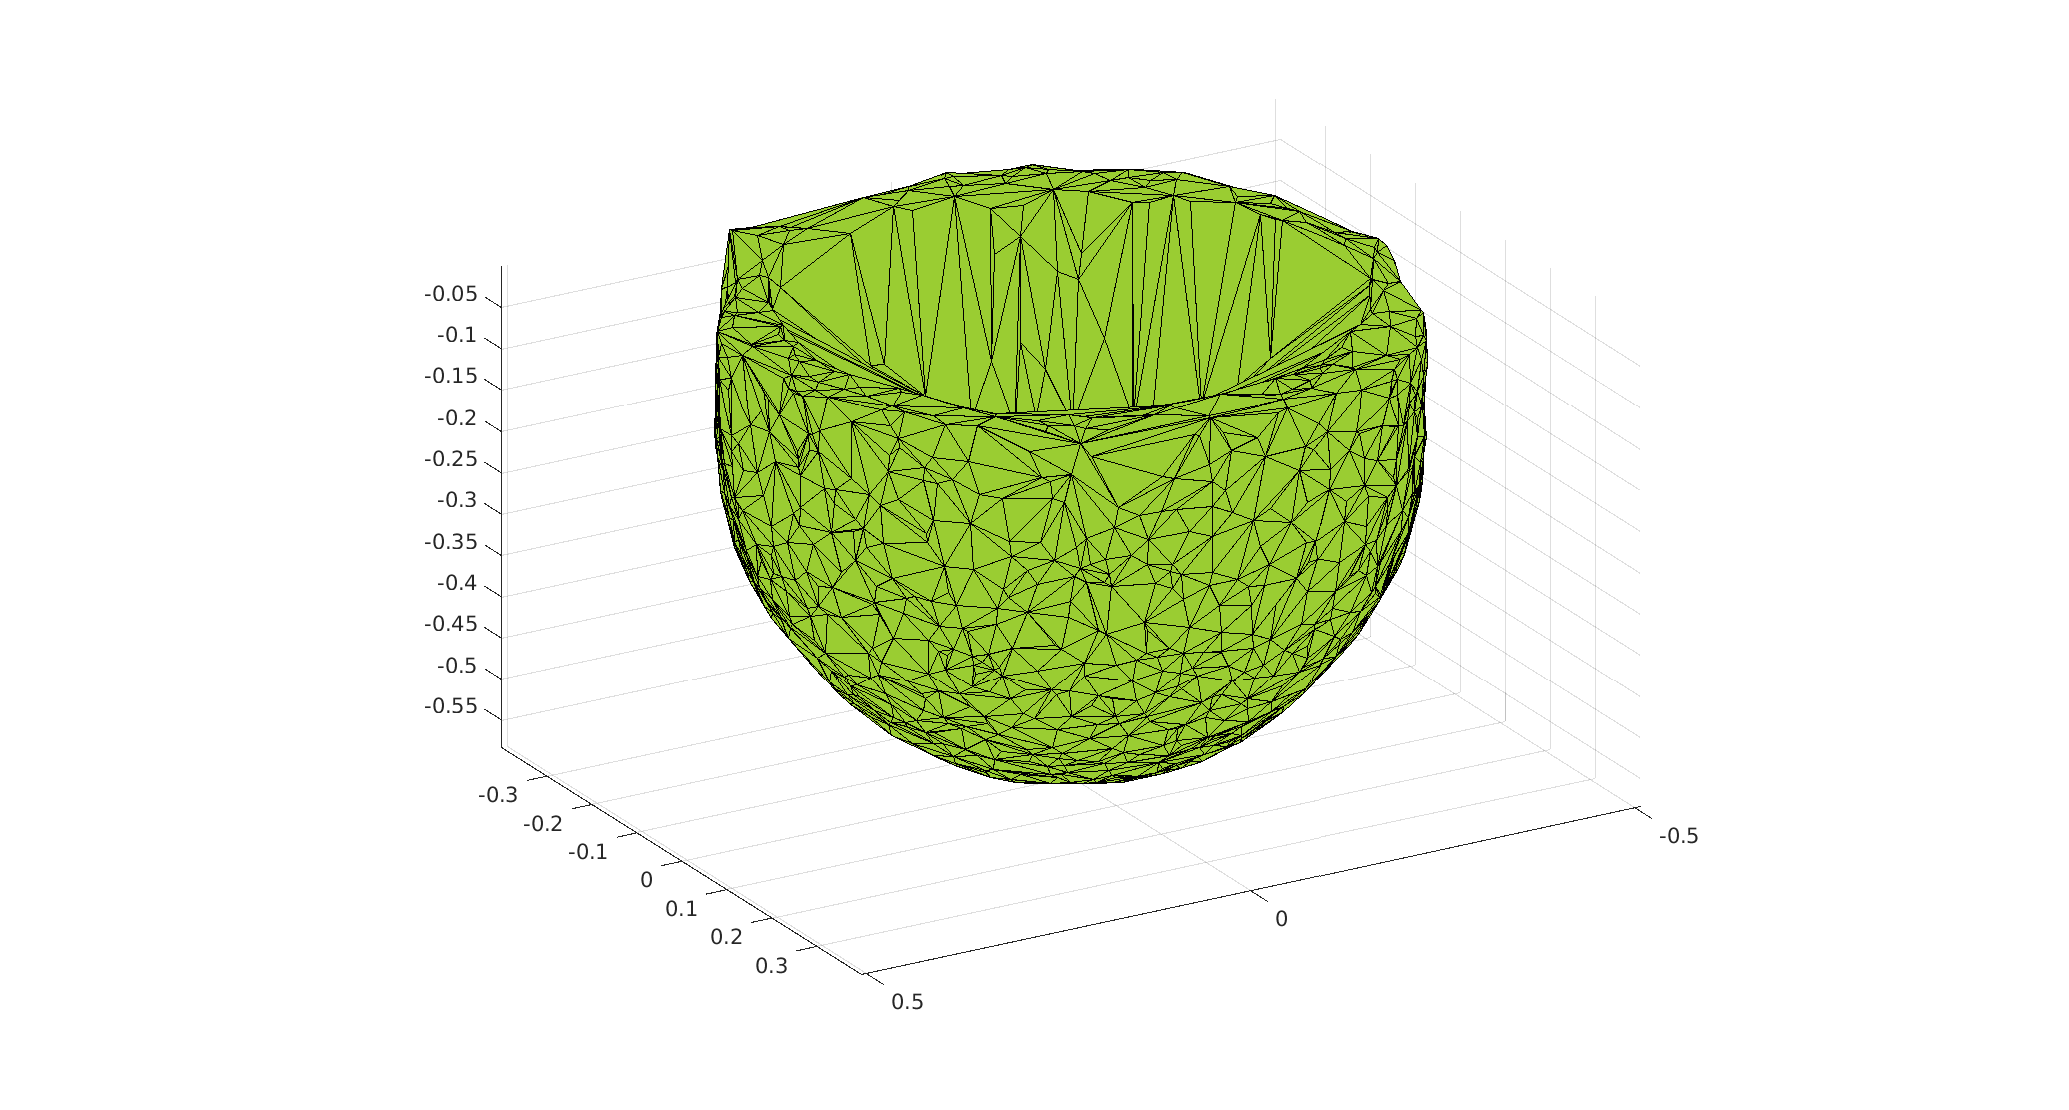
\includegraphics[width=.95\linewidth]{img/WorkSpaceDelta.eps}}
	\caption{A convex hull of the workspace of the Delta robot}
	\label{fig:Delta_WS}
\end{figure}
\end{frame}
%
\begin{frame}
\frametitle{Delta robot - Working volume}
In figure~\ref{fig:Delta_WS} a covex hull of the workspace of the Delta robot is reported. The surface has been generated as an $\alpha-shape$ \footfullcite{alpha-shape} with $r_\alpha = 0.2$.\\
The geometric figure gives an analytical instrument to validate a sound reference trajectory generation for the Delta kinematic.
\end{frame}
%
\subsection{Control}
\subsubsection{PD with gravity compensation}
\begin{frame}
\frametitle{PD with gravity compensation}
Control equation:
\begin{equation}
	\tau_{PD} = K_Pe + K_D\dot{e}+G(q)
\end{equation}
with
\[ K_P = 1500\,, \qquad K_D = 60\]
\end{frame}
%
\subsubsection{Computed torque}
\begin{frame}
\frametitle{Computed torque}
Control equation:
\begin{equation}
	\tau_{CT} = M(q)\ddot{q}_d + C(q,\dot{q})\dot{q} + G(q) + K_pe + K_v\dot{e}
\end{equation}
with
\begin{equation*}
K_P = 500, \; K_D = 100
\end{equation*}
\end{frame}
%
\begin{frame}
\frametitle{Computed torque}
%
\begin{columns}
\begin{column}{0.5\textwidth}
	Descrizione traiettoria
\end{column}
\begin{column}{0.5\textwidth}
	\begin{figure}
	\frame{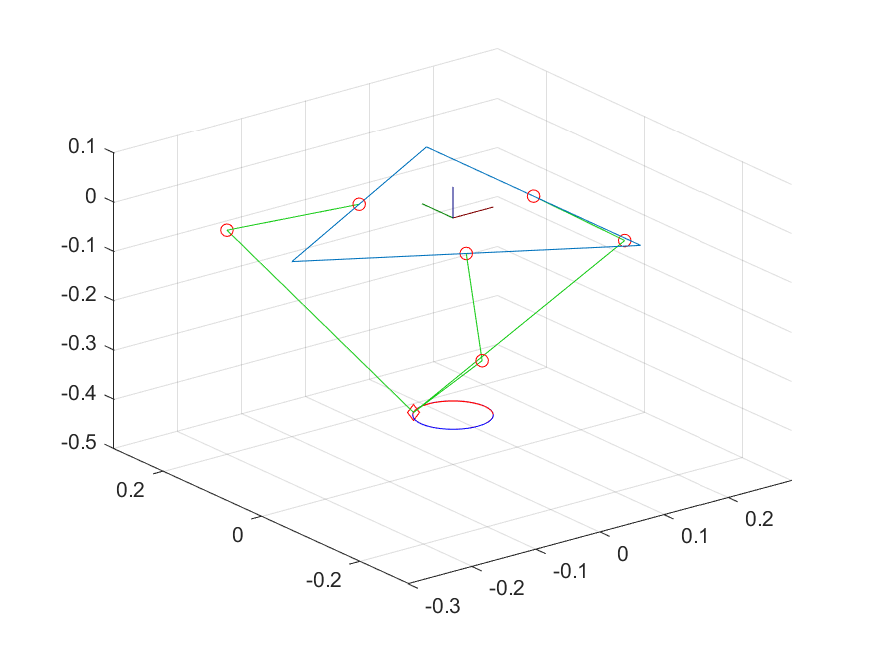
\includegraphics[width=\linewidth]{img/computedTorque/Visualizzatore.png}}
	\end{figure}
\end{column}
\end{columns}
\end{frame}
%
\begin{frame}
\frametitle{Computed torque}
%
\begin{columns}
	\begin{column}{0.5\textwidth}
	\begin{figure}
	\frame{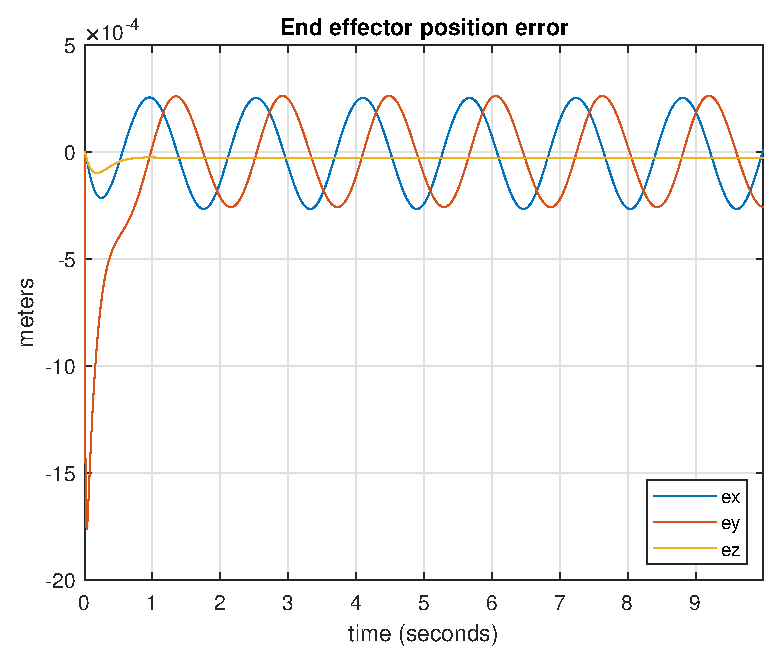
\includegraphics[width=\linewidth]{img/computedTorque/Eerror}}
	\end{figure}
	\end{column}
	%
	\begin{column}{0.5\textwidth}
	\begin{figure}
	\frame{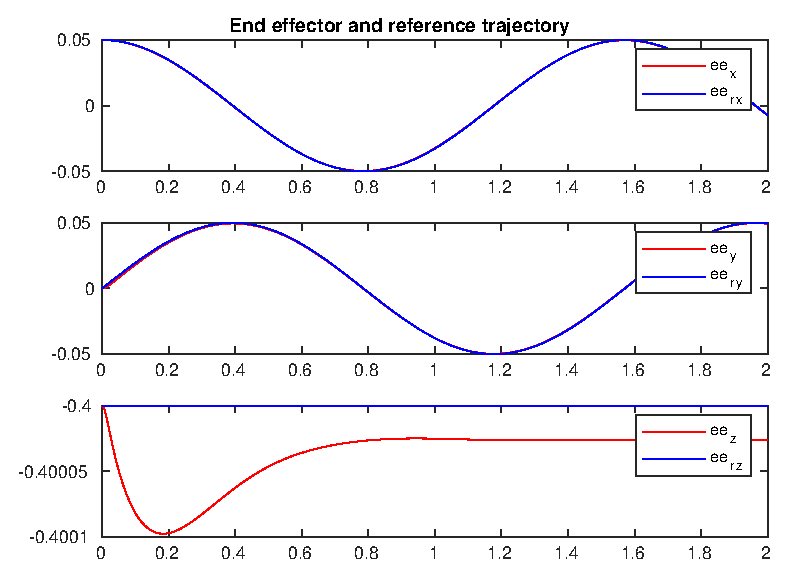
\includegraphics[width=\linewidth]{img/computedTorque/confronto}}
	\end{figure}
	\end{column}
\end{columns}
\end{frame}
%
\begin{frame}
\frametitle{Computed torque}
%
\begin{columns}
	\begin{column}{0.5\textwidth}
	\begin{figure}
	\frame{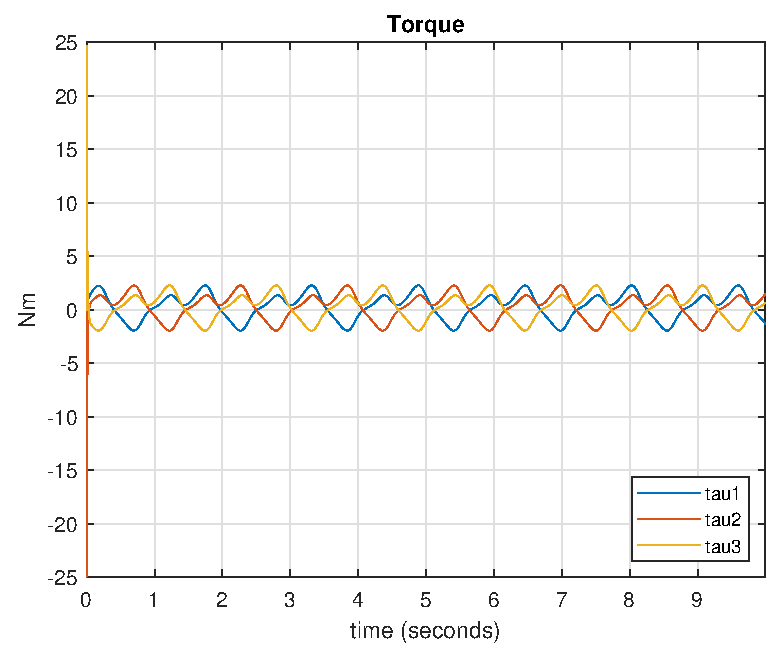
\includegraphics[width=\linewidth]{img/computedTorque/tau}}
	\end{figure}
	\end{column}
	%
	\begin{column}{0.5\textwidth}
	\begin{figure}
	\frame{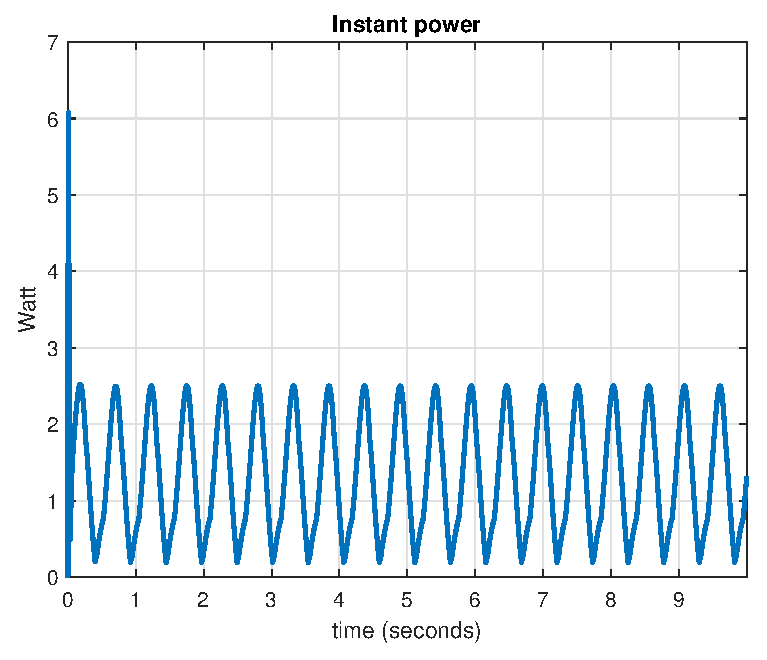
\includegraphics[width=\linewidth]{img/computedTorque/Power}}
	\end{figure}
	\end{column}
\end{columns}
\end{frame}
%
\subsubsection{Backstepping}
\begin{frame}
\frametitle{Backstepping}
Control equation:
\begin{equation}
	\tau_{BS} = M(q)\ddot{q}_r + C(q,\dot{q})\dot{q}_r + G(q) - K_ds + J^Te
\end{equation}
with
\begin{align*}
\ddot{q}_r=\ddot{q}_d - \Lambda\dot{e}, && \dot{q}_r=\dot{q}_d - \Lambda e, && s=\dot{q}_ - \dot{q}_r, && K_d=50, && \Lambda=400
\end{align*}
\end{frame}
%
\begin{frame}
\frametitle{Backstepping}
%
\begin{columns}
\begin{column}{0.5\textwidth}
	Descrizione traiettoria
\end{column}
\begin{column}{0.5\textwidth}
	\begin{figure}
	\frame{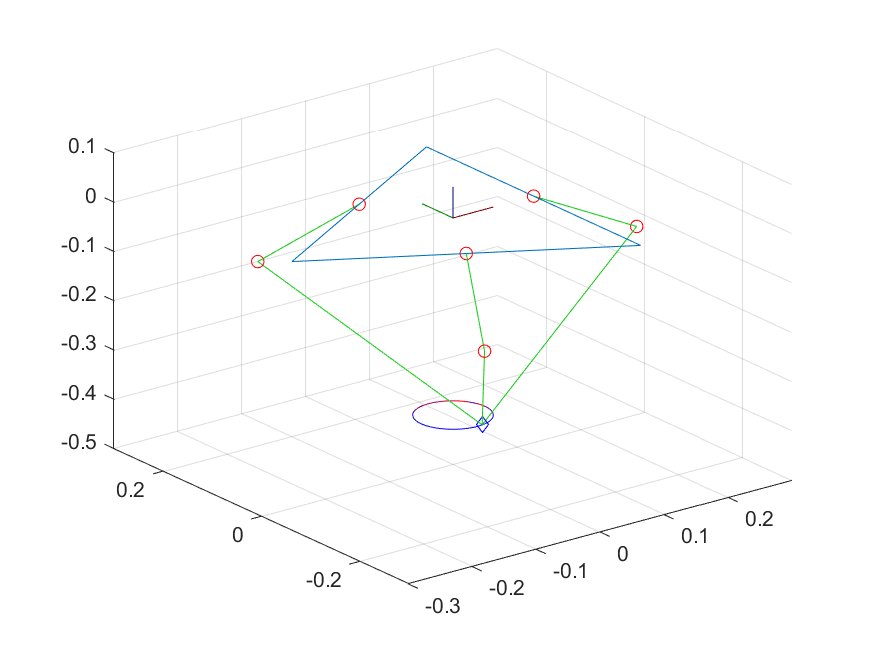
\includegraphics[width=\linewidth]{img/backstepping/Visualizzatore.png}}
	\end{figure}
\end{column}
\end{columns}
\end{frame}
%
\begin{frame}
\frametitle{Backstepping}
%
\begin{columns}
	\begin{column}{0.5\textwidth}
	\begin{figure}
	\frame{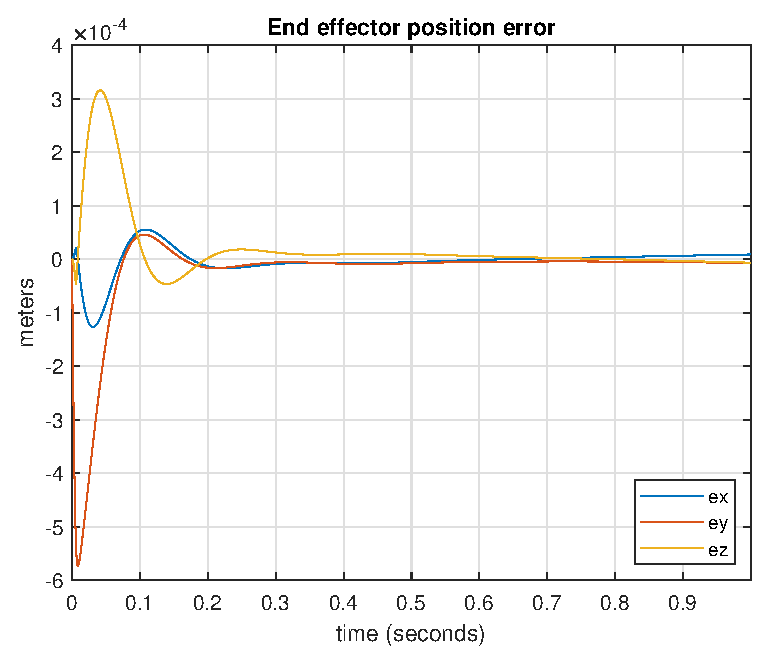
\includegraphics[width=\linewidth]{img/backstepping/Eerror}}
	\end{figure}
	\end{column}
	%
	\begin{column}{0.5\textwidth}
	\begin{figure}
	\frame{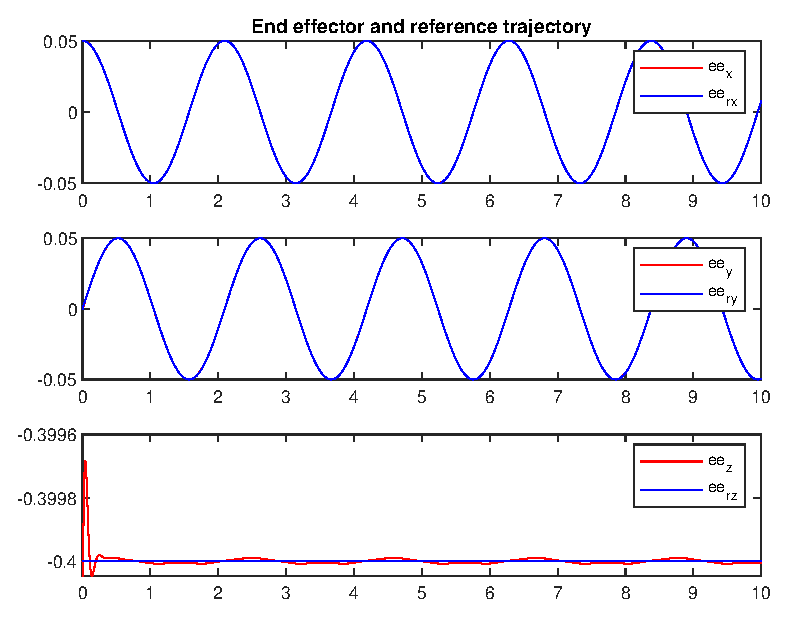
\includegraphics[width=\linewidth]{img/backstepping/confronto}}
	\end{figure}
	\end{column}
\end{columns}
\end{frame}
%
\begin{frame}
\frametitle{Backstepping}
%
\begin{columns}
	\begin{column}{0.5\textwidth}
	\begin{figure}
	\frame{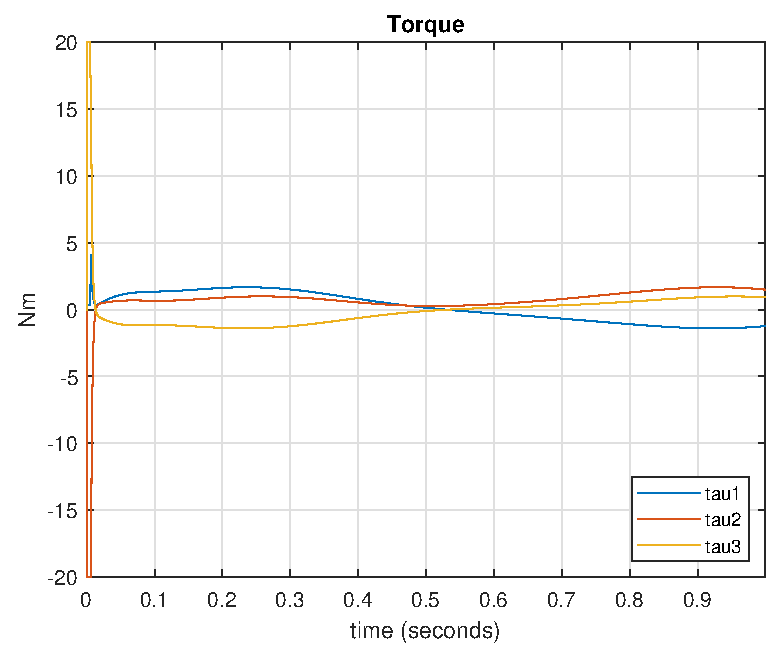
\includegraphics[width=\linewidth]{img/backstepping/tau}}
	\end{figure}
	\end{column}
	%
	\begin{column}{0.5\textwidth}
	\begin{figure}
	\frame{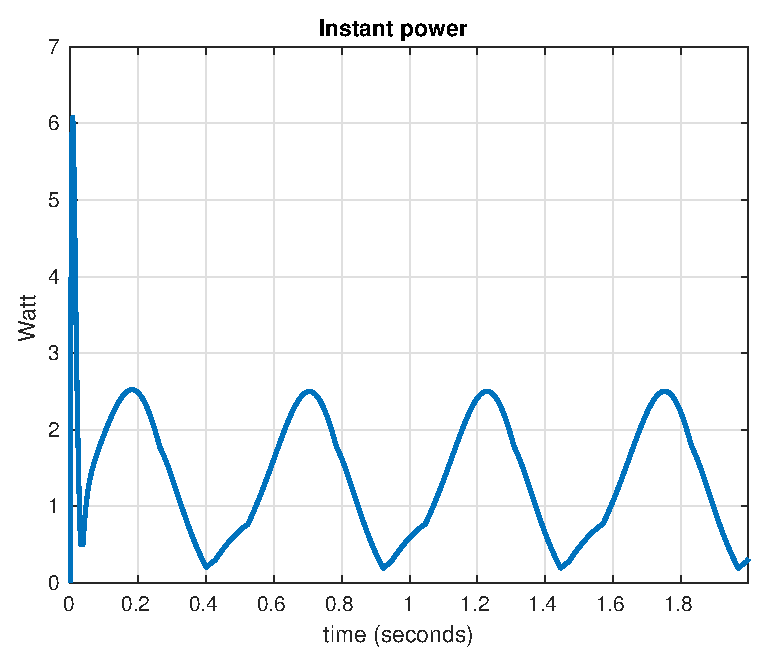
\includegraphics[width=\linewidth]{img/backstepping/Power}}
	\end{figure}
	\end{column}
\end{columns}
\end{frame}
%
%
\subsubsection{Adaptive backstepping}
\begin{frame}
\frametitle{Adaptive backstepping}
\end{frame}